
\begin{figure}[h]
  \centering      
    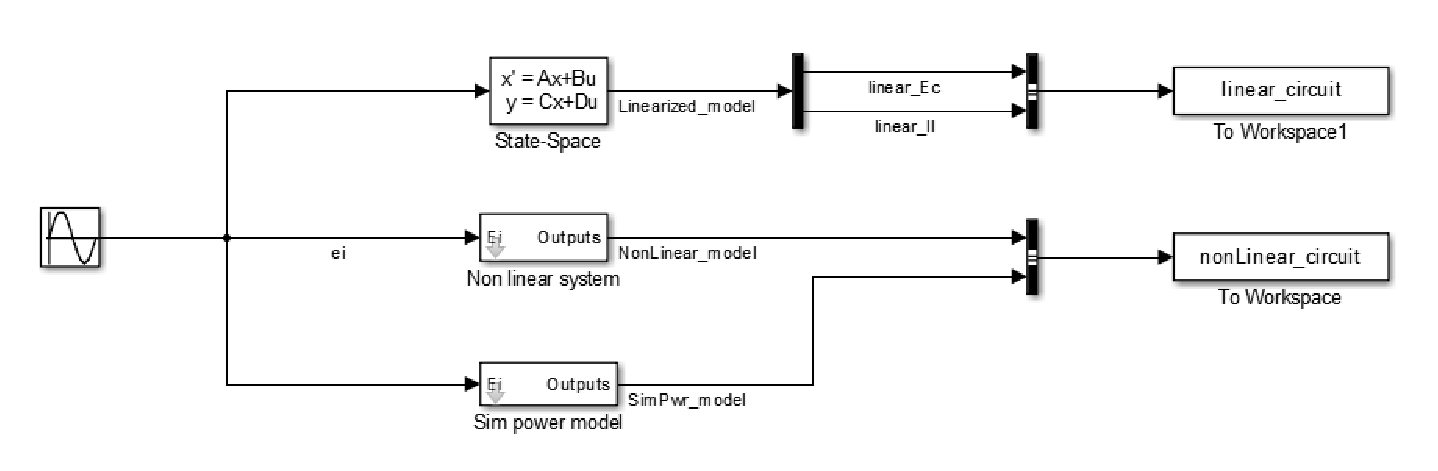
\includegraphics[width=1\textwidth]{Ex1_Simulink.eps}
	\caption{Simulink model used for electrical simulation and comparison}
\end{figure}


\begin{figure}[h]
  \centering      
    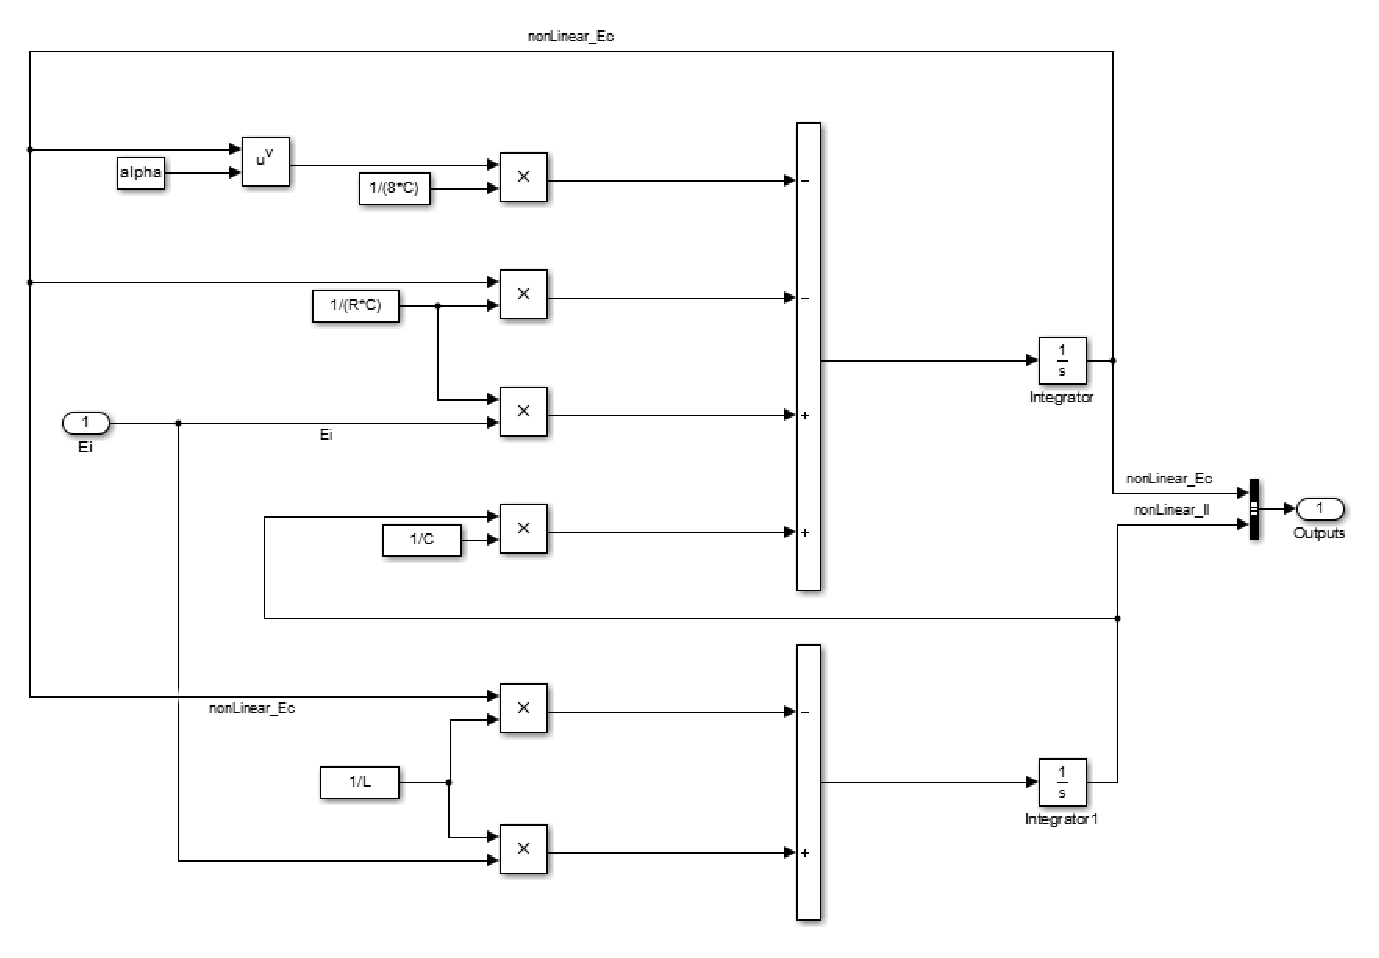
\includegraphics[width=1\textwidth]{Ex1_ExactModel.eps}
	\caption{Simulink model used for electrical exact non linear model simulation}
\end{figure}


\begin{figure}[h]
  \centering      
    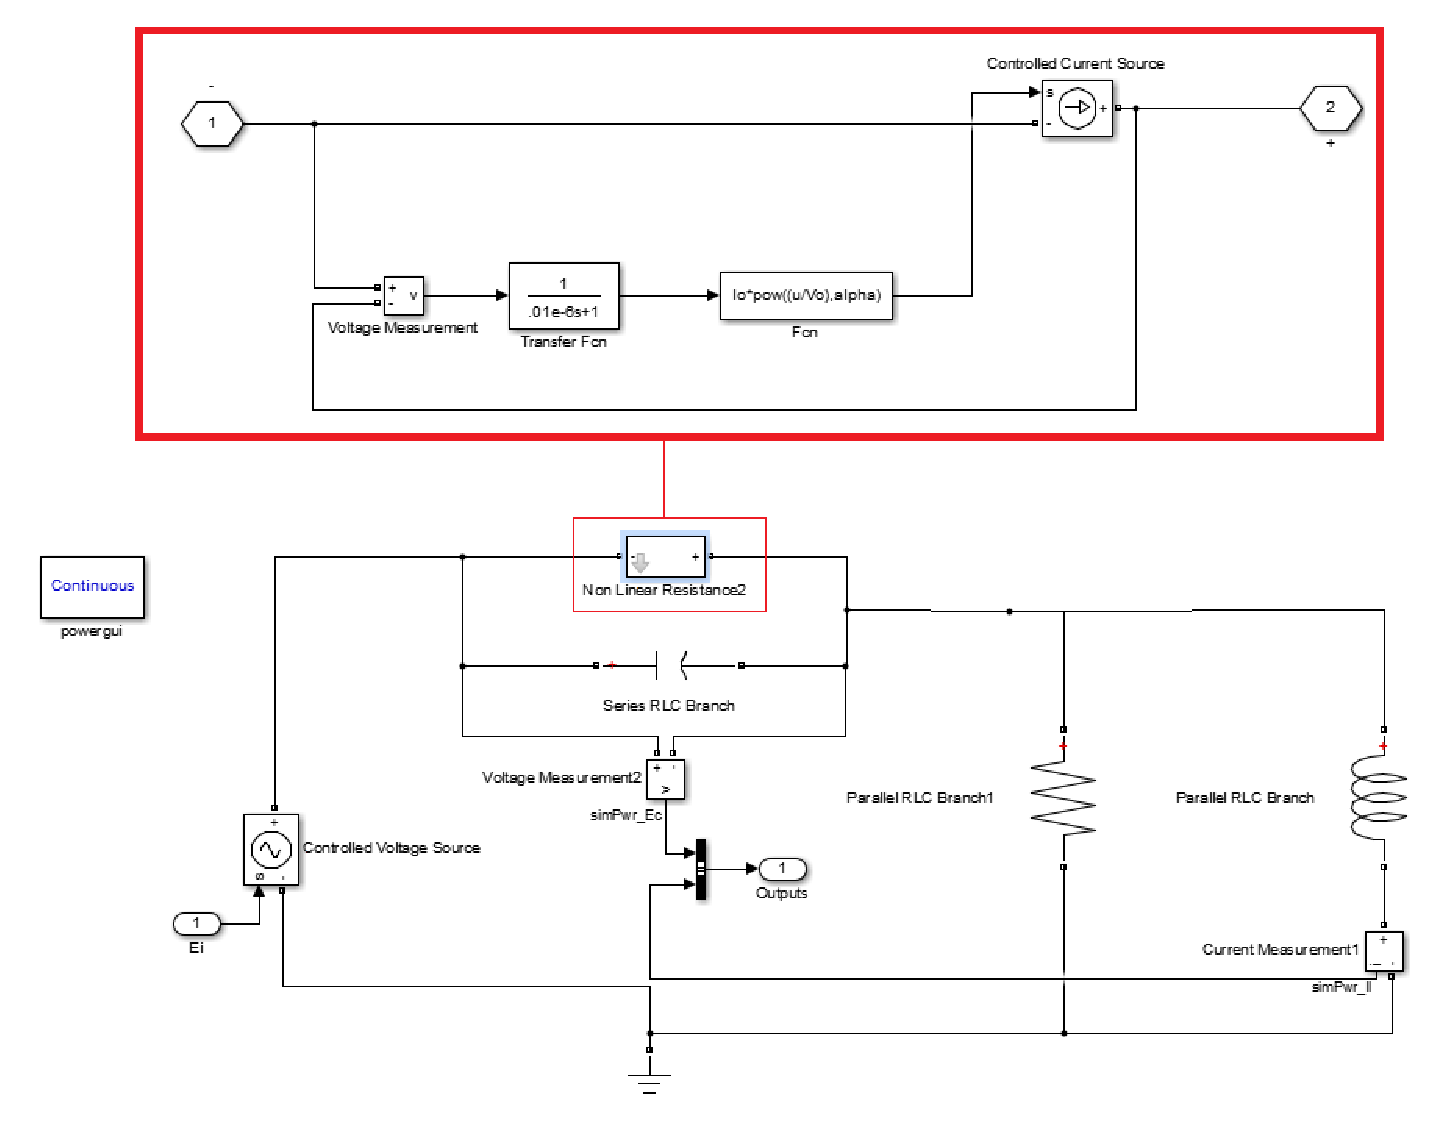
\includegraphics[width=1\textwidth]{Ex1_SimPower.eps}
	\caption{Simpower model used for electrical exact non linear model simulation}
\end{figure}

\begin{figure}[h]
  \centering      
    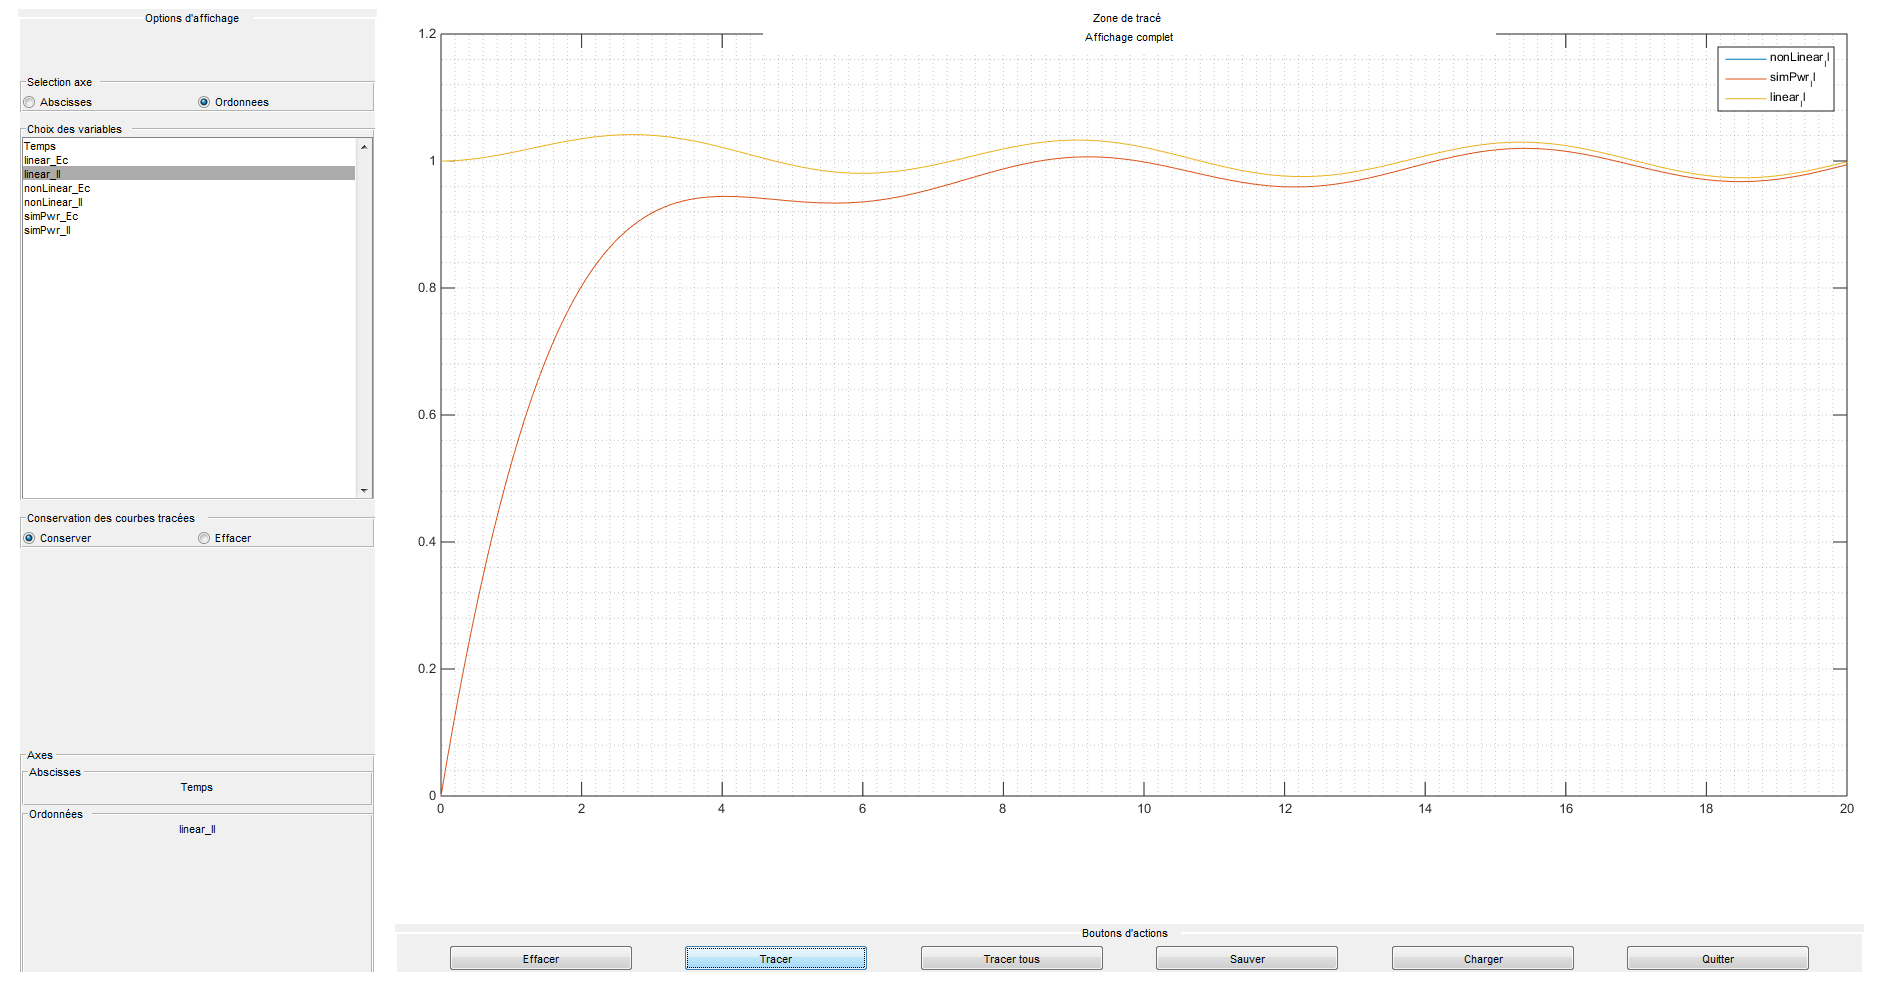
\includegraphics[width=0.8\textwidth]{Ex1_0dec1_Il.eps}
	\caption{Courbe d'intensit� au cours du temps avec A=0.1V}
\end{figure}

\begin{figure}[h]
    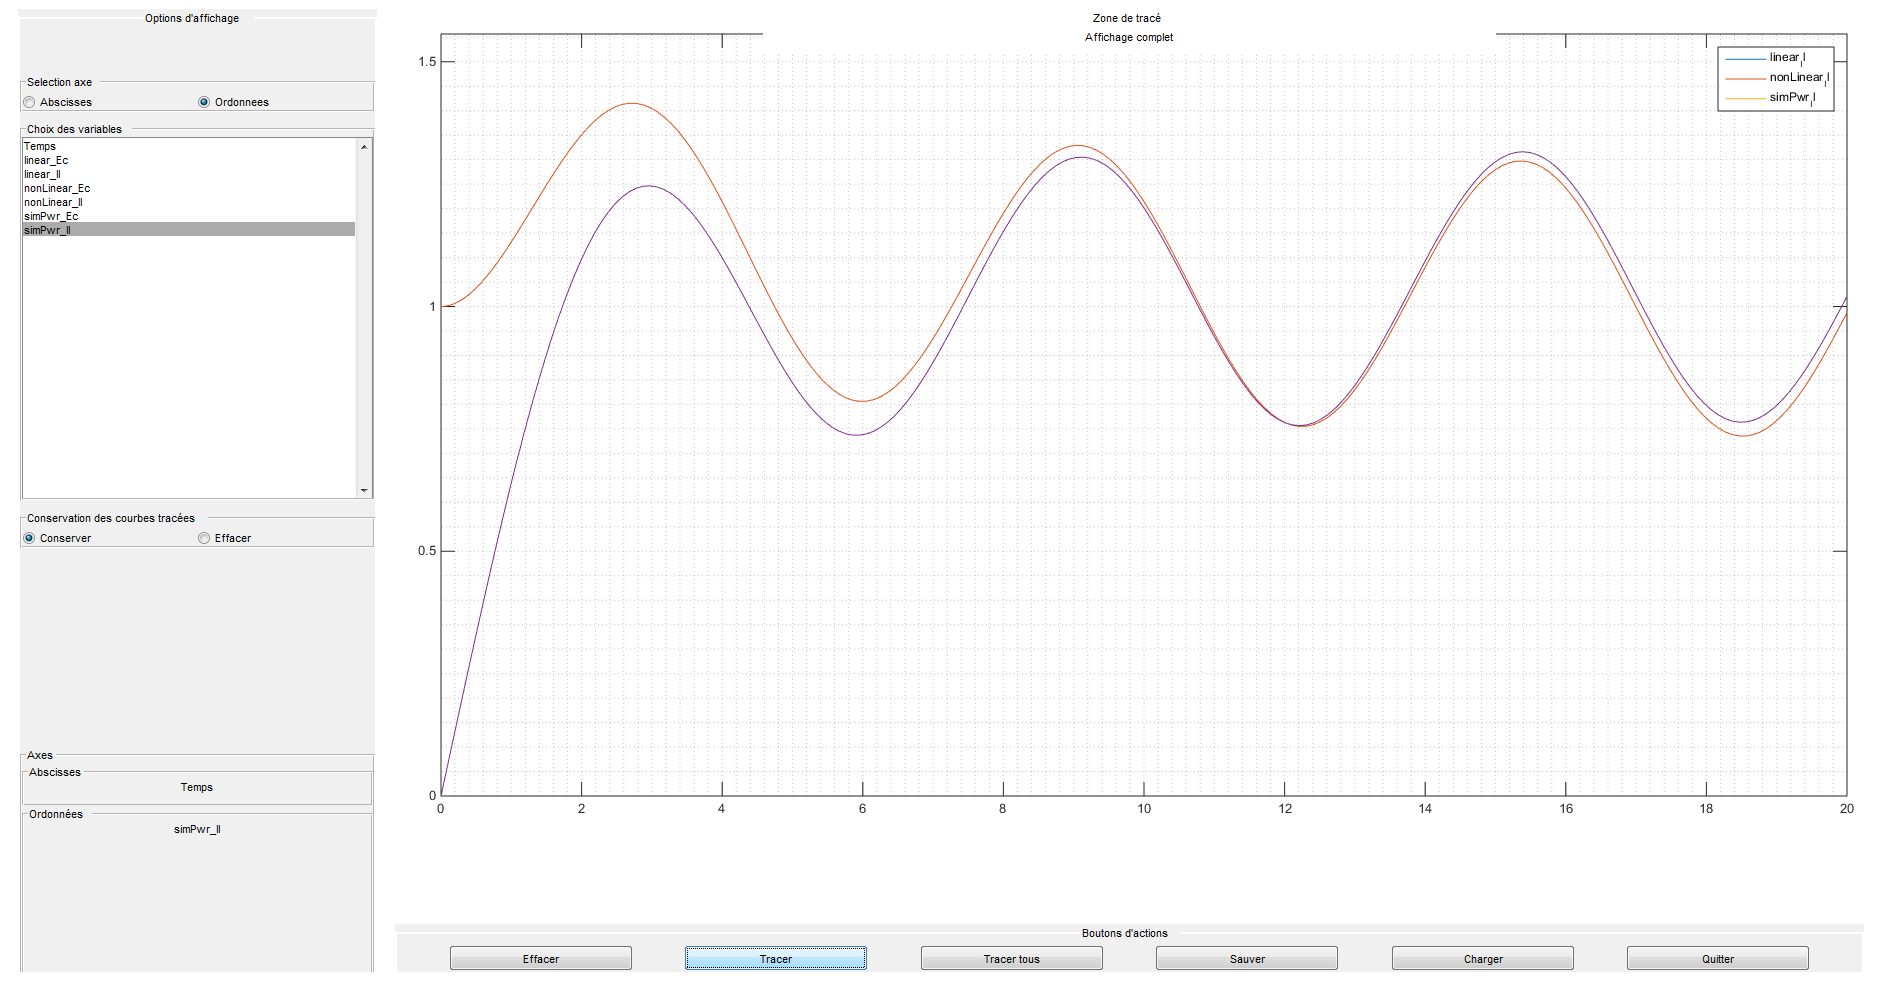
\includegraphics[width=0.8\textwidth]{Ex1_1_Il.eps}
	\caption{Courbe d'intensit� au cours du temps avec A=1V}
\end{figure}

\begin{figure}[h]
    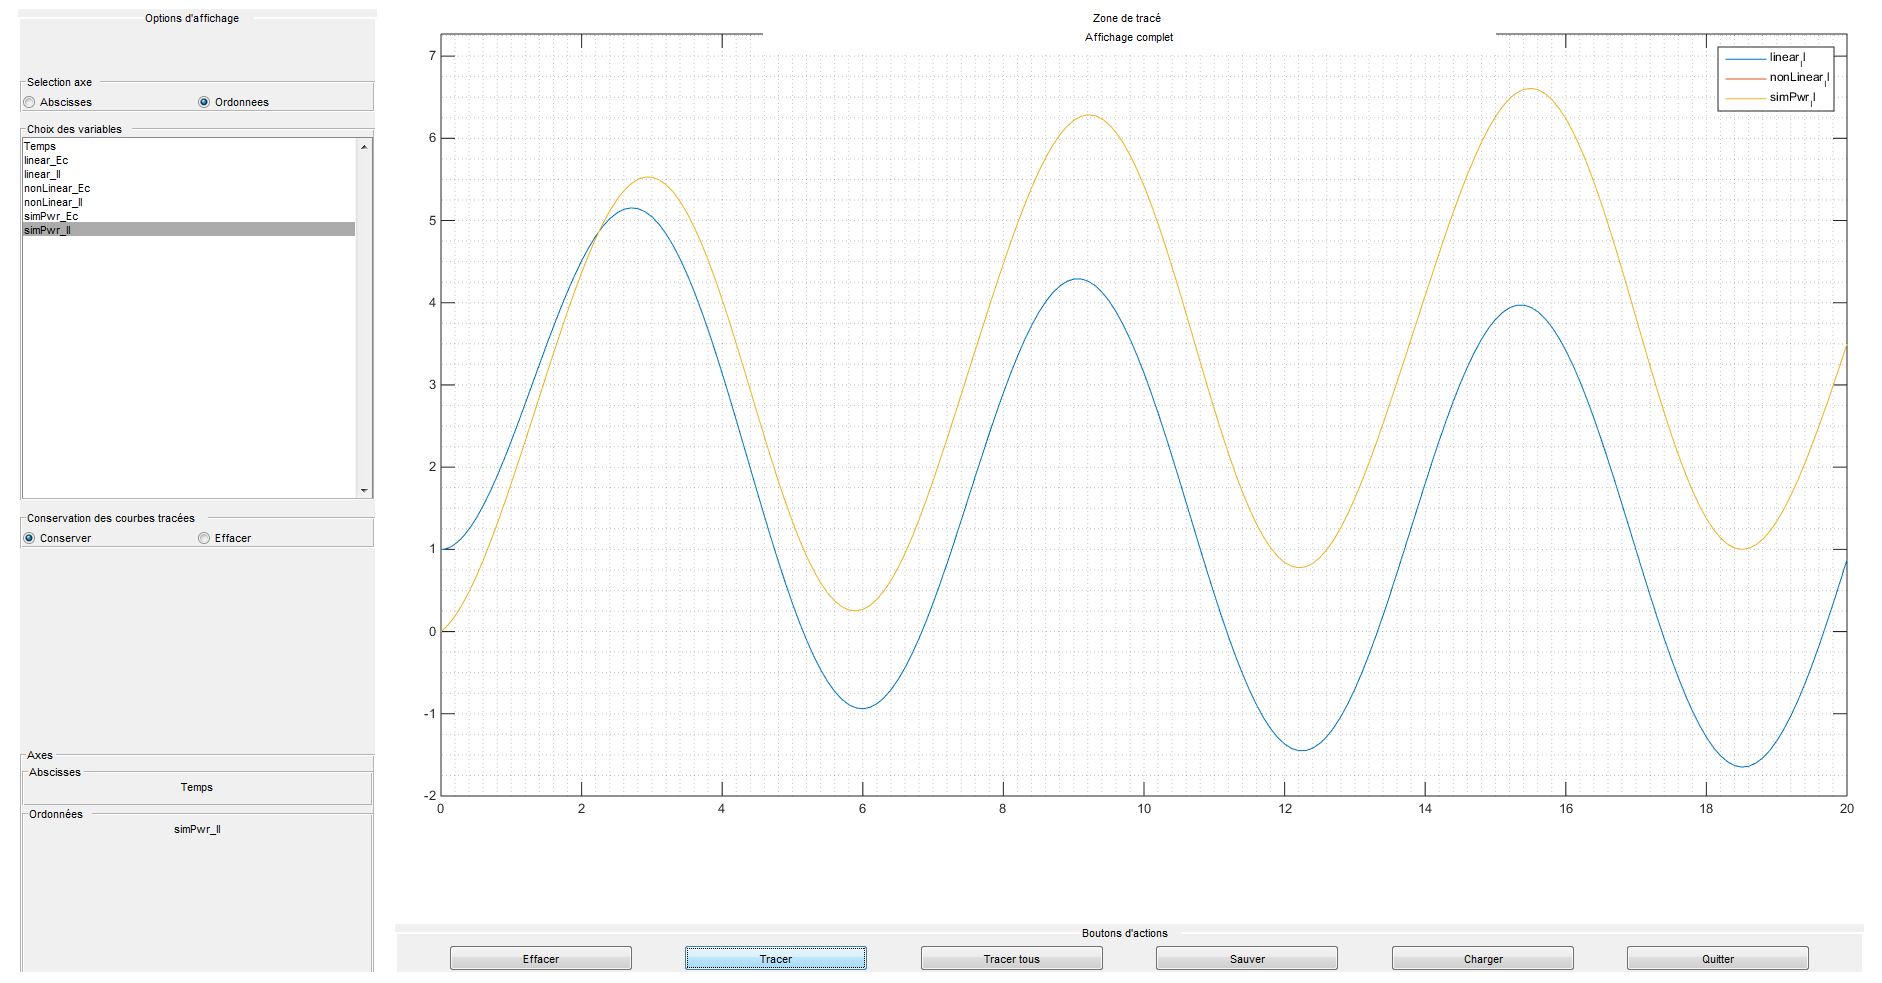
\includegraphics[width=0.8\textwidth]{Ex1_10_Il.eps}
	\caption{Courbe d'intensit� au cours du temps avec A=10V}
\end{figure}